% mnras_template.tex
%
% LaTeX template for creating an MNRAS paper
%
% v3.0 released 14 May 2015
% (version numbers match those of mnras.cls)
%
% Copyright (C) Royal Astronomical Society 2015
% Authors:
% Keith T. Smith (Royal Astronomical Society)

% Change log
%
% v3.0 May 2015
%    Renamed to match the new package name
%    Version number matches mnras.cls
%    A few minor tweaks to wording
% v1.0 September 2013
%    Beta testing only - never publicly released
%    First version: a simple (ish) template for creating an MNRAS paper

%%%%%%%%%%%%%%%%%%%%%%%%%%%%%%%%%%%%%%%%%%%%%%%%%%
% Basic setup. Most papers should leave these options alone.
\documentclass[a4paper,fleqn,usenatbib]{mnras}

% MNRAS is set in Times font. If you don't have this installed (most LaTeX
% installations will be fine) or prefer the old Computer Modern fonts, comment
% out the following line
%\usepackage{newtxtext,newtxmath}
% Depending on your LaTeX fonts installation, you might get better results with one of these:
%\usepackage{mathptmx}
%\usepackage{txfonts}

% Use vector fonts, so it zooms properly in on-screen viewing software
% Don't change these lines unless you know what you are doing
\usepackage[T1]{fontenc}
\usepackage{ae,aecompl}


%%%%% AUTHORS - PLACE YOUR OWN PACKAGES HERE %%%%%

% Only include extra packages if you really need them. Common packages are:
\usepackage{graphicx}	% Including figure files
\usepackage{amsmath}	% Advanced maths commands
\usepackage{amssymb}	% Extra maths symbols

%%%%%%%%%%%%%%%%%%%%%%%%%%%%%%%%%%%%%%%%%%%%%%%%%%

%%%%% AUTHORS - PLACE YOUR OWN COMMANDS HERE %%%%%

% Please keep new commands to a minimum, and use \newcommand not \def to avoid
% overwriting existing commands. Example:
%\newcommand{\pcm}{\,cm$^{-2}$}	% per cm-squared

%%%%%%%%%%%%%%%%%%%%%%%%%%%%%%%%%%%%%%%%%%%%%%%%%%

%%%%%%%%%%%%%%%%%%% TITLE PAGE %%%%%%%%%%%%%%%%%%%

% Title of the paper, and the short title which is used in the headers.
% Keep the title short and informative.
\title[Predicting extragalactic distance errors]{Predicting extragalactic distance errors using Bayesian inference in multi-measurement catalogs}

% The list of authors, and the short list which is used in the headers.
% If you need two or more lines of authors, add an extra line using \newauthor
\author[G. Chaparro-Molano et al.]{Germ\'an Chaparro-Molano,$^{1}$\thanks{E-mail: gchaparrom@ecci.edu.co}
Juan Carlos Cuervo,$^{2}$
Oscar Alberto Restrepo Gait\'an$^{1,3}$ \newauthor
Sergio Torres Arzay\'{u}s$^{4}$
\\
% List of institutions
$^{1}$Vicerrector\'ia de Investigaci\'on, Universidad ECCI, 111311 Bogot\'a, Colombia\\
$^{2}$Department, Institution, Street Address, City Postal Code, Country\\
$^{3}$Radio Astronomy Instrumentation Group, Universidad de Chile, Santiago de Chile, Chile\\
$^{4}$Centro Internacional de F\'isica, Bogot\'a, Colombia
}

% These dates will be filled out by the publisher
\date{Accepted XXX. Received YYY; in original form ZZZ}

% Enter the current year, for the copyright statements etc.
\pubyear{2015}

% Don't change these lines
\begin{document}
\label{firstpage}
\pagerange{\pageref{firstpage}--\pageref{lastpage}}
\maketitle

% Abstract of the paper
\begin{abstract}
This is a simple template for authors to write new MNRAS papers.
The abstract should briefly describe the aims, methods, and main results of the paper.
It should be a single paragraph not more than 250 words (200 words for Letters).
No references should appear in the abstract.
\end{abstract}

% Select between one and six entries from the list of approved keywords.
% Don't make up new ones.
\begin{keywords}
Galaxies: distances -- keyword2 -- keyword3
\end{keywords}

%%%%%%%%%%%%%%%%%%%%%%%%%%%%%%%%%%%%%%%%%%%%%%%%%%

%%%%%%%%%%%%%%%%% BODY OF PAPER %%%%%%%%%%%%%%%%%%

\section{Introduction}


%Efforts to reduce the uncertainty in the estimate the Hubble constant are single-method such as SNIa \citet{hubsn2018}.
%Bayesian analysis of systematic uncertainties for cosmology when using SNIa-derived galactic parameters (heterogeneous errors) \citet{unity}. 
%Hubble constant MCMC estimation based on Cepheids distance determination for NGC 4258 \citet{hubngc}. 
%\citet{hub2010} is the important hubble paper, although the original hubble estimation from redshift independent distances is \citet{huborig}. 
%\citet{ridsn} estimates distances using SNIa but no redshifts. 
%\citet{riess} is the 2.4 percent determination of hubble constant. 
%Changes in Hubble constant estimation using TF relation without Cepheids \citet{noceph}.
%GW searches \citet{gwgallist}, we should improve redshift independent distance determination .
%Determining the spatial distribution of galaxies in order to study large-scale structure \citet{gallargescale} or local universe peculiar velocities \citet{localunipv}. Kinematics of nearby galaxies in void \citet{void}
%\citet{6df} attempt to predict redshift-derived distance errors within a Bayesian framework yields 26\%.
%Studies of anisotropy be it of morphological types \citet{morphanis} or density-velocity \citet{nongauss}
%Determining whether a galaxy belongs to a group by analyzing their common properties \citet{gg3500} with conclusions regarding the halo mass function
%Anisotropy hubble from HST data \citet{anishub} and from NED-D \citet{tecciencia}. 
%10\% estimated uncertainty for photometrically derived distance scale ladder \citet{hubunc}.
%\citet{locunivcf} local universe structure reconstruction Cosmicflows-1
%\citet{precisetf} corrected the TF method for uncertainties in galaxy inclinations. \citet{tf07dist}
%  \citet{said} has used emcee for Tully-Fisher in the southern Zone of Avoidance.
%\citet{hyperleda} does not give a prescription for error estimation.

% UNUSED - which also need to take into account instrument detection limits \citet{catmatch} and source identification \citet{baymatch}. Importance of distance and catalogs \citet{catetg,catspi} in: Exploration of prior discrepancy modeling in model estimation \citet{priordisc}

Understanding the uncertainties in redshift-independent extragalactic distance measurements is absolutely necessary before reporting statistically sound conclusions regarding the structure of the local universe \citep{void,locunivcf,nongauss,6df,localunipv,said,gg3500}, large scale structure \citep{anishub,gallargescale,morphanis,tecciencia,bayesh}, and events like transient gravitational wave detections \citep{gwgallist}. Hubble constant estimations have been using increasingly sophisticated statistical tools for primary distance determination methods, such as SNIa \citep{ridsn,unity,hubsn2018}, Cepheids \citet{hubngc} or both \citep{riess}. Although most estimates of the Hubble constant use Cepheid calibration for calibrating secondary methods \citep{hubunc,huborig,hub2010}, \citet{noceph} have explored changes in Hubble constant estimation using the Tully-Fisher relation (TF) relation without Cepheid calibration. Secondary methods for extragalactic distance determination like the TF relation, or the Fundamental Plane (FP) have recently become more precise thanks to increasing volumes of data from surveys like 6dF \citep{6df}  and  2MASS \citep{2mass,tf07dist} together with Spitzer data \citep{sorce}, along with improved statistical methods \citep{precisetf}. \\

As of 2018, three multi-measurement catalogs including a substantial amount of redshift-independent extragalactic distance measurements have been released: HyperLEDA \citep{hyperleda}, NED-D \citep{ned07,ned}, and Cosmicflows-3 \citep{cosmicflows}. HyperLEDA includes a homogenized catalog for extragalactic distances in the nearby universe, with 12866 distance measurements for 518 galaxies to date. NED-D is the NASA/IPAC Extragalactic Distance catalog of Redshift-Independent Distances, which compiles XXX distance measurements for XXX galaxies, for which  $\sim1800$ galaxies ($\sim1$\%) have more than 12 distance measurements, and $~180$ galaxies ($\sim0.1$\%) have distance measurements using more than 6 different methods. Cosmicflows-3 is the most up-to-date catalog, which reports distance measurements for 10616 galaxies for up to four distance determination methods, and calibrated with supernova luminosities. However, unlike HyperLEDA or NED-D, Cosmicflows-3 only reports the latest distance measurement for each method. In HyperLEDA, NED-D and Cosmicflows-3 errors are reported as one standard deviation from the reported distance modulus. Treatment of errors for combining distance moduli across methods or across measurements is suggested by \citet{ned07} and \citet{cosmicflows} to be based on weighted estimates such as the uncertainty of the weighted mean, albeit with caution due to the hererogeneous origin of the compiled data. In the case of NED-D, this is complicated by the fact that many errors are not reported or are reported as zero. In fact, the TF relation method has the largest number of galaxies with non-reported distance modulus errors (818 to date). Even though extragalactic distances measured using the TF relation were originally reported to have a relative error in distance modulus of $10-20$\% \citep{tforig}, we consider that this conservative estimate can be improved upon by using a predictive model based on the distance error of galaxies that use the same distance determination method. This requires a robust estimation of the variance of extragalactic distances based on the available data.\\

For many galaxies in all three catalogs, the random error for each distance modulus measurement $\epsilon_i$ (for $i=1,...,N$, for $N$ distance measurements per galaxy) is not representative of the scatter across measurements, even when considering the same method for determining distances. In addition, distance modulus distributions for each measurement (which are assumed to be Gaussian) are transformed to log-normal distributions in metric distance space. We improve upon previous methods by robustly estimating the underlying variance across measurements and distance determination methods for the three catalogs by bootstrap sampling the posterior distribution of each extragalactic distance \citep{chaparro18}, and comparing our results to more commonly used frequentist methods, such as the weighted estimates mentioned above. Furthermore, we build a predictive Bayesian model for the 818 galaxies in the NED-D catalog whose distances were measured using the TF relation but have non-reported errors.\\

%$\sim16000$ galaxies ($\sim9$\%) have more than one distance measurement,

Here go the sections.

% is CF in NED-D? cite number of methods per catalog? important to add to appendix supplementary figures to complement the multi-method analysis for hyperleda, all ned-d and cosmicflows. say that we made new data tables? create plots for those tables. also try quadrature model with zero setting systematic error?


%All papers should start with an Introduction section, which sets the work in context, cites relevant earlier studies in the field by \citet{photred2}, and describes the problem the authors aim to solve \citep[e.g.][]{photred1}.



\section{Posterior distribution for extragalactic distances}
\label{sec:post} % used for referring to this section from elsewhere
 
As mentioned in the Introduction, the best approach to consider the effects of random and scattering errors in catalog-wide, multi-method distance analyses is to perform a robust estimation of the variance of the posterior distribution of each extragalactic distance. The posterior distribution of the distance to a given galaxy can be obtained by drawing distance modulus samples from $P(\mu)$, which is the unweighted mixture of normal distributions corresponding to each distance modulus measurement $\mu_i$,
\[\mu\sim\sum_i^N \mathcal{N}(\mu_i,\epsilon_i^2)\ ,\]
and then converting to metric distance,
\[D=10^{\frac{\mu}{5}+1}\ .\]
Therefore,
\[D_G\sim\sum_i^N\mathrm{lognormal}(M_i,\sigma_{M_i}^2)\ .\]
Here $M_i=\ln D_i$ and $\sigma_{M_i}=\epsilon_i\cdot\ln10$.\\

However, this method is not very efficient for a standardized treatment of errors. It is more convenient to treat each extragalactic metric distance $D_G$ as a normal random variable with a single-valued $\sigma_D$ as a measure of the uncertainty in the estimation of an extragalactic distance,
\[D_G\sim \mathcal{N}(D,\sigma_D^2)\]
For this reason we compare four methods for estimating the $D,\,\sigma_D$ pair. Two of these methods (H, M) use robust measures of the posterior distribution of each extragalactic distance, and the other two (P, Q) use measures based on propagation of errors.

\subsection{Estimating the variance of $P(D_G)$}
\label{sec:meth} 

Method H takes $D$ as the median of the posterior and $\sigma_D$ as the half-distance (H) between the 84th and 16th percentiles of the posterior. Method M takes $D$ as the median of the posterior and $\sigma_D$ as the median absolute deviation (MAD) of the posterior. Method P consists on calculating $D$ from the weighted mean distance modulus $\bar{\mu}^*$ with weights $w_i=\epsilon_i^{-2}$. $\sigma_D$ is calculated by propagation (P) of measurement errors  i.e. from the uncertainty of the weighted mean \citep{cosmicflows},
\begin{equation}
\sigma_D^P=0.461\,\bar{D}^*\,\left(\sum_i^Nw_i\right)^{-1/2} \ ,
\end{equation}
Method P does not take into account the scatter in distance measurements for single galaxies, which is why method Q calculates $D$ same as method P, but $\sigma_D$ is calculated as the sum in quadrature (Q) of the propagated uncertainty of the weighted mean and the propagated unbiased weighted sample variance $\sigma_D^*$:
\begin{equation}
\sigma_D^Q=\left[ \left(\sigma_D^P\right)^2+\Big(\sigma_D^*\Big)^2\right]^{1/2} \ .
\end{equation}
Here $\sigma^*_D$ is calculated as  \citep{wstdev},
\begin{equation}
\sigma^*_D=0.461\,\bar{D}^*\,\sqrt{\frac{N}{N-1.5}\frac{\sum_i^Nw_i(\mu_i-\bar{\mu}^*)^2}{\sum_i^Nw_i}}\ .
\end{equation}
If the P and Q methods, which are not robust, are representative of the variance of the posterior, they should yield similar results as the H method. Next section shows that this is not the case.

\subsection{Comparison of variance estimation methods}
\label{sec:comp} 


Without loss of generality, we will focus on galaxies whose distances have been measured using the Tully-Fisher method in the NED-D catalog because it is the method with the most non-reported errors in the database. From here on, when we mention distance measurements in the NED-D catalog, we will be excluding from our analysis measurements that require the target redshift to calculate the distance, as indicated in the \texttt{redshift (z)} field. \\

Even though our analysis for error estimation can be used to combine distance measurements using different methods for single galaxies, we think that it is more meaningful to separate the analysis by method. A full discussion of our error estimation method applied to multi-method measurements in the HyperLEDA, NED-D and Cosmicflows-3 is given in the appendix.\\

Fig.~\ref{fig:comp} shows that the center and variance of the posterior distribution of each extragalactic distance is best explained using the H method, whereas the less robust P and Q methods under-predict the variance for galaxies in the whole distance range. The M method also under-predicts the variance, but being a robust method, it is not as sensitive to outliers as the mehods P and Q, as seen in the case of NGC 1558 in Fig.~\ref{fig:comp}. For the more symmetrical posterior distribution of UGC 12792, the M and Q methods predict the same center and variance. \\

\begin{figure*}

	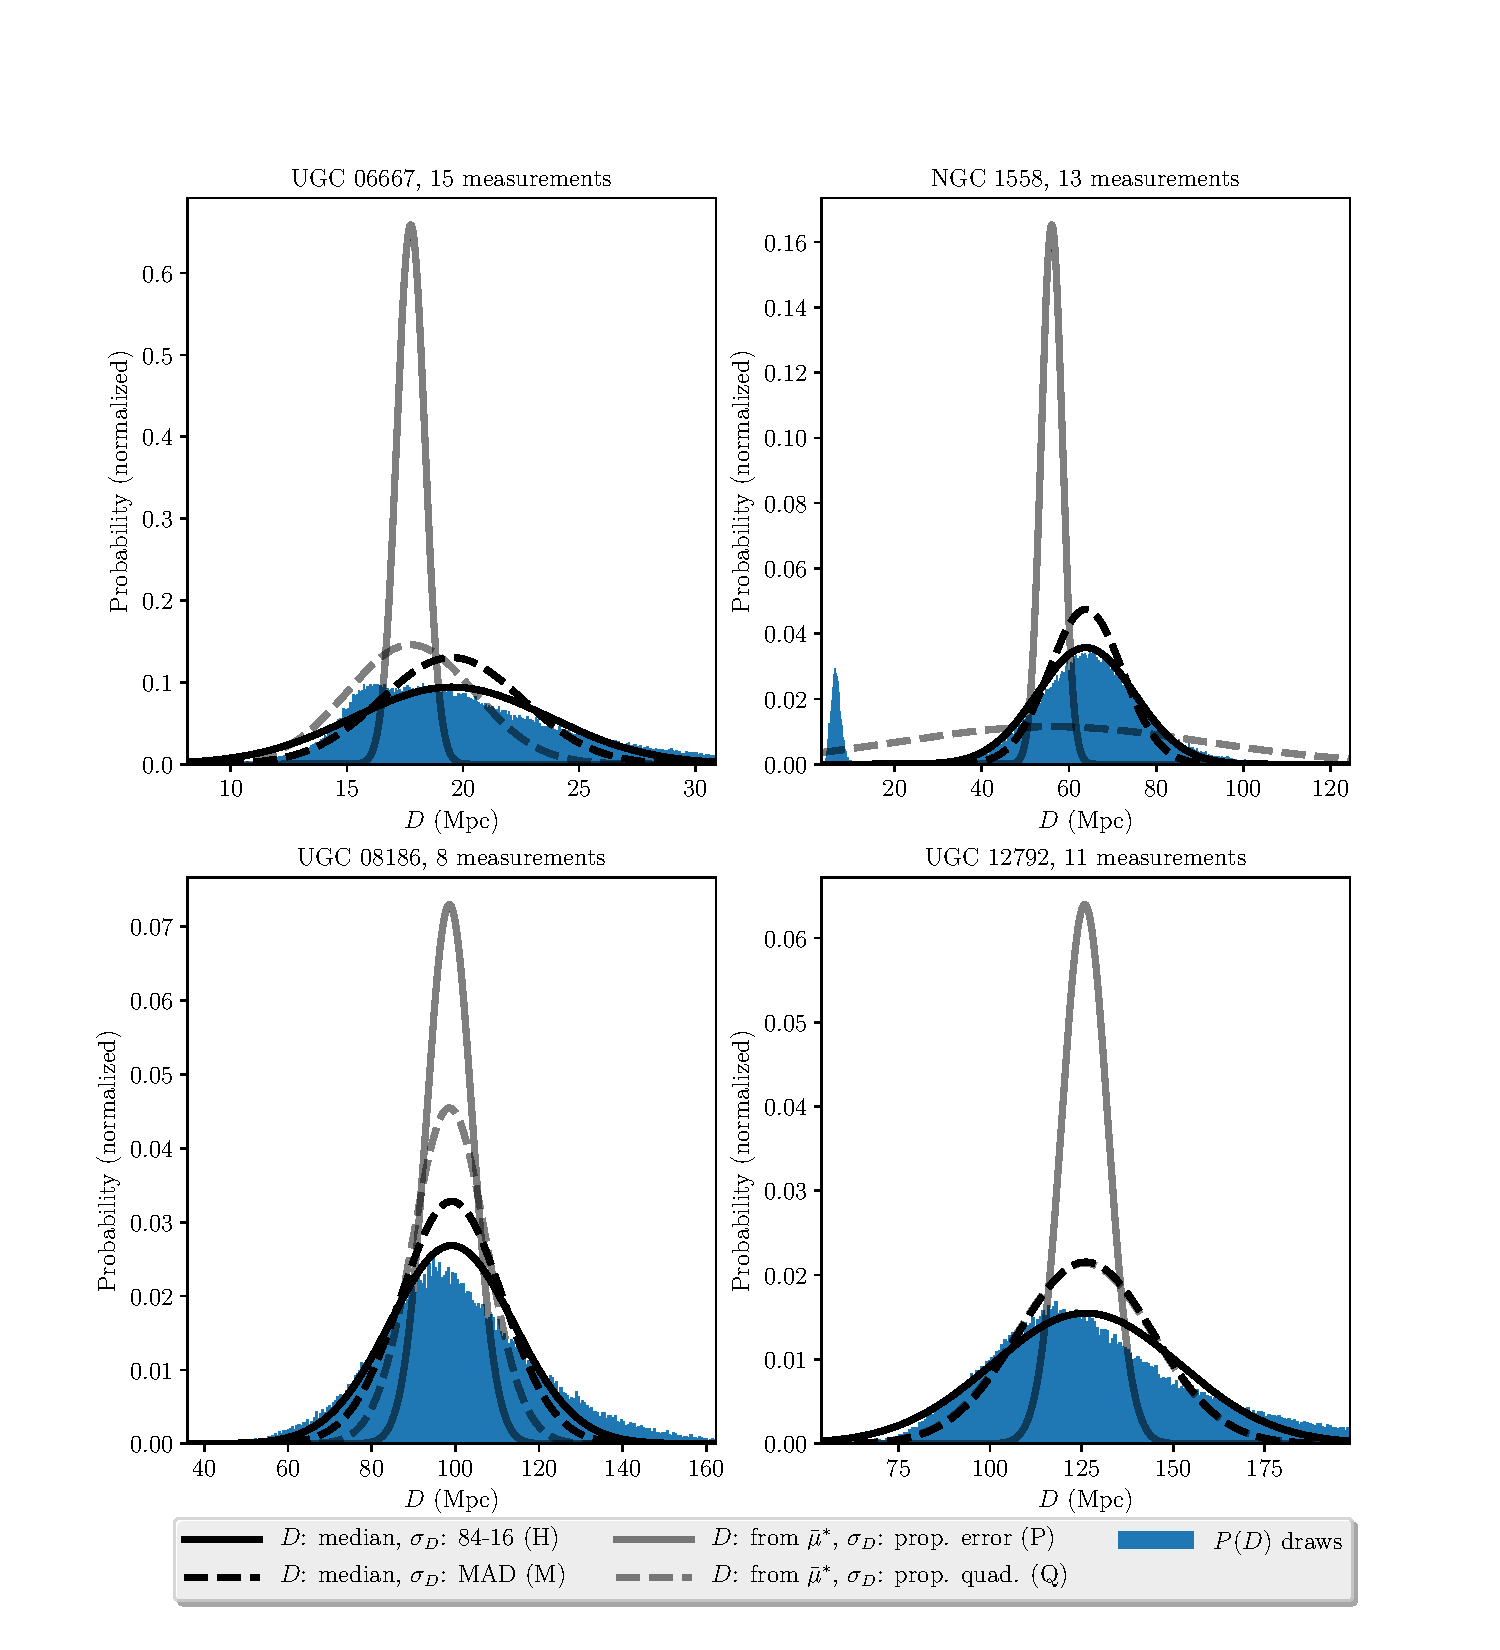
\includegraphics[scale=0.7]{comp}
    \caption{Comparison of extragalactic distance posterior distribution draws and modeled distributions for UGC 06667, NGC 1558, UGC 08186, and UGC 12792 using the Tully-Fisher Method for distance determination in NED-D. The four methods used for approximating the posterior distribution (H, M, P, and Q) are described in the text. }
    \label{fig:comp}
\end{figure*}

\begin{figure}

	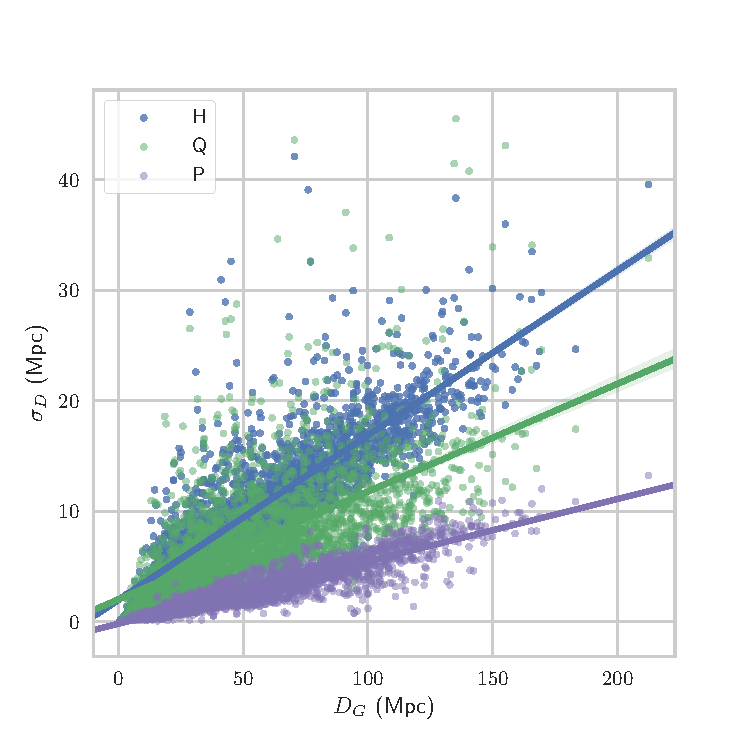
\includegraphics[scale=0.7]{hqp}
    \caption{Median extragalactic distance vs. predicted extragalactic distance errors for galaxies with more than 5 TF distance measurements in NED-D according to the H, Q, P error models, showing a linear regression and confidence intervals computed using the \texttt{seaborn.regplot} Python function.}
    \label{fig:hqp}
\end{figure}

\begin{figure}

	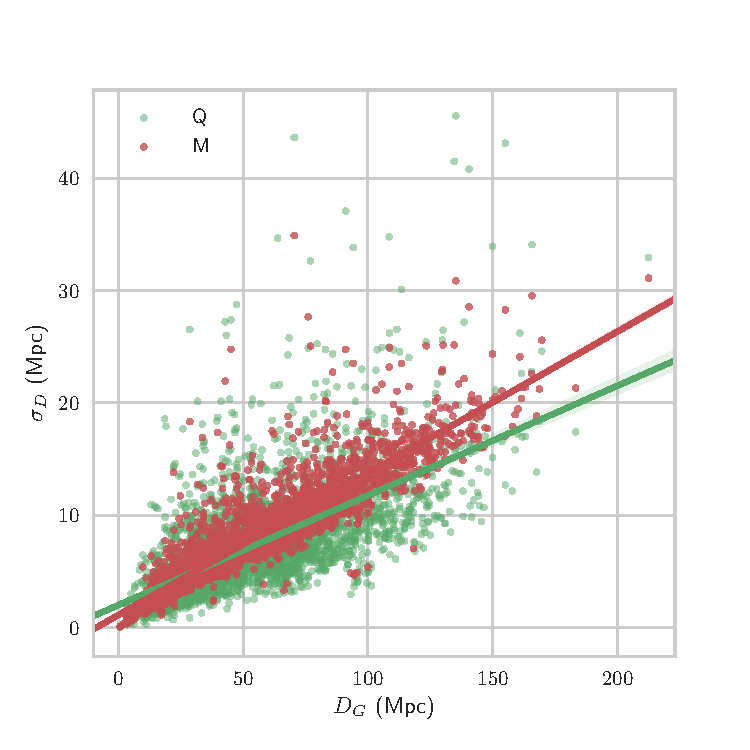
\includegraphics[scale=0.7]{qm}
    \caption{Median extragalactic distance vs. predicted extragalactic distance errors for galaxies with more than 5 TF distance measurements in NED-D according to the Q, M error models, showing a linear regression and confidence intervals computed using the \texttt{seaborn.regplot} Python function.}
    \label{fig:qm}
\end{figure}

\begin{figure}

	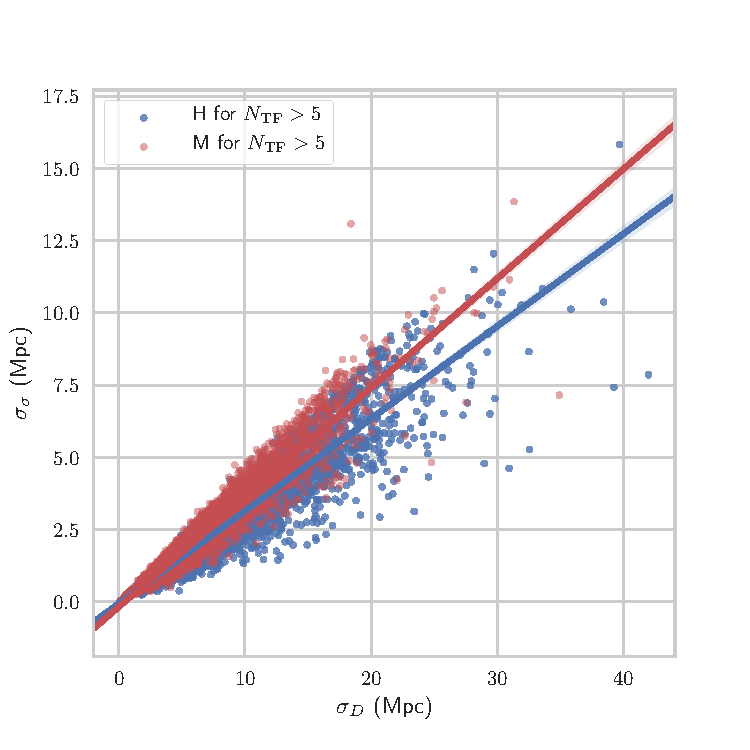
\includegraphics[scale=0.7]{ee}
    \caption{Predicted extragalactic distance errors vs. variance of the error as determined by the H and M methods, showing a linear regression and confidence intervals computed using the \texttt{seaborn.regplot} Python function. }
    \label{fig:ee}
\end{figure}

Distance errors grow linearly with distance, as seen in Fig.~\ref{fig:hqp}. This means that there is a strong systematic component in the variance of $P(D_G)$. Furthermore, the quadrature (Q) and propagation (P) methods underpredict distance errors for most galaxies in the sample. Fig.~\ref{fig:qm} shows that method Q underpredicts distance errors with respect to the median absolute deviation method (M), which also shows a tighter linear correlation due to its robustness.\\

Given that $\sigma_D$ calculated using the H method is obtained from many realizations from the posterior distribution of extragalactic distances, it is also possible to calculate its variance as the half-distance between the 84th and 16th percentile of $\sigma_D$ realizations. Fig.~\ref{fig:ee} shows that the variance of the estimated error is proportional to the error for the H and M methods. This will be relevant in Section~\ref{sec:predbay} when we construct a predictive model for non-reported errors.

\section{Predictive Bayesian Models for missing errors}
\label{sec:predbay} % used for referring to this section from elsewhere

As seen in Figs.~\ref{fig:hqp} and \ref{fig:qm}, TF distance errors estimated using the robust methods H and M grow in a roughly linear fashion with distance, but are randomly distributed around this trend line. For this reason we try out several Bayesian models in order to be able to predict missing distance errors. For this, we use the \texttt{emcee} affine invariant Markov Chain Monte Carlo (MCMC) ensemble sampler \citep{emcee}. Recently, \texttt{emcee} has been proved to be useful in obtaining probabilistic estimations for photometric redshifts \citet{photred1,photred2}. Since we want to be able to predict non-reported errors, our model selection is based on posterior predictive checks, i.e. we rely on models that can create synthetic datasets similar to the original dataset \citep{gelmanppd}. This allows us to reproduce the original variance of the error (Fig.~\ref{fig:ee}. Many Bayesian analyses often do not use posterior predictive checks, like in the work of \citet{propprob2018} and \citet{bayesh}, where they used \texttt{emcee} for posterior sampling, and using Bayesian and Akaike Information Criteria along with Bayes factors for model assessment, but without attempting to reproduce the original variance of the data. This is also the case in other Bayesian tools like LINMIX  \citep{gmastro}, which is widely used in astronomy for approximating unobserved data.  \\

First we assume that for a galaxy $j$ the distance error $\sigma_{Dj}$ is a random normal variable, with variance $\sigma_{\sigma j}$ and mean $\hat{\sigma}_{Dj}$, 
\begin{equation}
P(\sigma_{Dj}|\hat{\sigma}_{Dj},\sigma_{\sigma j})=\mathcal{N}(\hat{\sigma}_{Dj},\sigma_{\sigma j}^2)\ .
	\label{eq:prob}
\end{equation}
Our likelihood function is the joint probability that each of the $\sigma_D=\{\sigma_{Dj}\}$ in the original dataset of $m$ galaxies is generated by the above probability,  
\begin{equation}
 P(\sigma_{D}|\hat{\sigma}_{D},\sigma_{\sigma})=\prod_j^mP(\sigma_{Dj}|\hat{\sigma}_{Dj},\sigma_{\sigma j})
\end{equation}
We want to test the hypothesis mentioned above that all errors and their variances $(\hat{\sigma}_D=\{\hat{\sigma}_{Dj}\},\ \sigma_\sigma=\{\sigma_{\sigma j}\})$ can be estimated from a single model depending on the extragalactic distances $D_G=\{D_{Gj}\}$ and a set of distance-independent parameters $\pmb{\theta}$. Thus the likelihood can be expressed as,
\[P(\sigma_D|D_G,\pmb{\theta})=\prod_j^mP(\sigma_{Dj}|D_{Gj},\pmb{\theta})\ .\]
Following Bayes' theorem we can compute the posterior probability up to a constant,
\[P(\pmb{\theta}|D_G,\sigma_D)\propto P(\pmb{\theta})P(\sigma_D|D_G,\pmb{\theta})\ .\]
Due to the simplicity of the models used here, we will only use conservative (flat) priors. From our analysis of Fig.~\ref{fig:ee}, all our models take $\sigma_\sigma=f\sigma_D$, where $f$ is one of the parameters in $\pmb{\theta}$. On the other hand, our models will differ by the proposed functional forms of $\hat{\sigma}_D(D_G,\pmb{\theta})$.\\

We obtain a computationally credible sampling of the posterior probability by removing the burn-in steps of the random walk according to the autocorrelation time. We can then create synthetic datasets by drawing a parameter sample $\pmb{\theta}_k$ from the posterior and using it to draw from the likelihood to create a new dataset, i. e. drawing new $\sigma_{Dj,s}$ from the probability distribution for all galaxies in the original dataset using equation~\ref{eq:prob}. We then assess the validity of the model by comparing synthetic data with the observed (i. e. original) data. This comparison is done by using a discrepancy measure $\mathcal{D}(\sigma_D|\pmb{\theta}_k)$ between data and model-derived expected values for the same data $e=\{e_j(\pmb{\theta}_k)\}$, where $\theta_k$ is drawn from the posterior distribution and $\sigma_D$ can be the observed errors or the model-generated synthetic errors. The discrepancy can be calculated using a statistic like $\chi^2$ \citep{chi2ms,otherdisc}, but here we will work with the Freeman-Tukey discrepancy since it is weight independent \citep{brooks}, 
\[\mathcal{D}(\sigma_D|\pmb{\theta}_k)=\sum_j^m(\sqrt{\sigma_{Dj}\vphantom{e_j(\pmb{\theta}_k)}}-\sqrt{e_j(\pmb{\theta}_k)})^2\]
For each parameter draw $k$, it is possible to compare the symulated discrepancy with the observed discrepancy. If the model is representative of the data, then for many parameter draws, the symulated and observed discrepancies should be similar. We can then calculate a Bayesian ``$p$-value'' as the ratio of ``draws when the observed discrepancies are larger than the synthetic discrepancies'' to ``total draws''. If this Bayesian $p$-value is too close to 0 or to 1 we can reject the model, otherwise we cannot reject the model, as it is generating synthetic data that is similar to the original data. This is better visualized using a discrepancy plot, where for each draw $k$, a synthetic discrepancy is paired with its corresponding observed discrepancy. If the discrepancy points are roughly equally distributed about the $\mathcal{D}_\mathrm{obs}=\mathcal{D}_\mathrm{sym}$ line, then we cannot reject the model.\\


Our first model is based on the (somewhat naive) hypothesis that there are are distinct systematic and random contributions to the distance measurement error, both of which are normally distributed. For this reason they are added in quadrature, 
\[\sigma_D^2=\sigma_s^2+\sigma_r^2\ .\]
If the systematic error is a scale factor error as Fig.~\ref{fig:hqp} suggests, $\sigma_r=sD$ where the scale factor $s$ and the random error $\sigma_r$ are independent of the distance. We then use \texttt{emcee} to sample the posterior over the parameter set $\pmb{\theta}=(f,s,\sigma_r)$. 

Several models in order to reach a predictive model. Central limit theorem?

\citet{gelman2003} and \citet{ppcinf} and for using posterior predictive checks for inference and prediction

%explicitly write priors

%Figures are referred to as e.g. Fig.~\ref{fig:example_figure}, and tables as
%e.g. Table~\ref{tab:example_table}.



% Example table
\begin{table}
	\centering
	\caption{This is an example table. Captions appear above each table.
	Remember to define the quantities, symbols and units used.}
	\label{tab:example_table}
	\begin{tabular}{lccr} % four columns, alignment for each
		\hline
		A & B & C & D\\
		\hline
		1 & 2 & 3 & 4\\
		2 & 4 & 6 & 8\\
		3 & 5 & 7 & 9\\
		\hline
	\end{tabular}
\end{table}


\section{Conclusions}

Discrepancy plots should be more widely used 

\section*{Acknowledgements}

The authors would like to thank O. L. Ram\'irez-Su\'arez and J. E. Forero-Romero for their valuable input during the early stages of this work. This research has made use of the NASA/IPAC Extragalactic Database (NED), which is operated by the Jet Propulsion Laboratory, California Institute of Technology, under contract with the National Aeronautics and Space Administration.

%%%%%%%%%%%%%%%%%%%%%%%%%%%%%%%%%%%%%%%%%%%%%%%%%%

%%%%%%%%%%%%%%%%%%%% REFERENCES %%%%%%%%%%%%%%%%%%

% The best way to enter references is to use BibTeX:

\bibliographystyle{mnras}
\bibliography{savedrecs} % if your bibtex file is called example.bib


% Alternatively you could enter them by hand, like this:
% This method is tedious and prone to error if you have lots of references
%\begin{thebibliography}{99}
%\bibitem[\protect\citeauthoryear{Author}{2012}]{Author2012}
%Author A.~N., 2013, Journal of Improbable Astronomy, 1, 1
%\bibitem[\protect\citeauthoryear{Others}{2013}]{Others2013}
%Others S., 2012, Journal of Interesting Stuff, 17, 198
%\end{thebibliography}

%%%%%%%%%%%%%%%%%%%%%%%%%%%%%%%%%%%%%%%%%%%%%%%%%%

%%%%%%%%%%%%%%%%% APPENDICES %%%%%%%%%%%%%%%%%%%%%

\appendix

\section{Some extra material}

If you want to present additional material which would interrupt the flow of the main paper,
it can be placed in an Appendix which appears after the list of references.

%%%%%%%%%%%%%%%%%%%%%%%%%%%%%%%%%%%%%%%%%%%%%%%%%%


% Don't change these lines
\bsp	% typesetting comment
\label{lastpage}
\end{document}

% End of mnras_template.tex